\chapter{绪论}\label{chap:intro}
\markboth{第一章\ \ 绪论}{}

\section{背景和意义}\label{sec:background}

\subsection{研究背景}\label{sec:background}

自动调制识别(Automatic Modulation Recognition, AMR)是一种用于识别无线电信号尤其是非合作信号的调制模式的技术。其目的是在缺少先验信息的情况下,自动检测无线通信信号的调制方式。这一技术在认知无线电、频谱感知、信号监视、干扰识别等多个领域中发挥着关键作用,并且近年来吸引了研究者的广泛关注。随着频谱环境日益复杂,认知无线电被视为解决严重频谱拥堵问题的有前途的方案,它依赖于自动调制识别技术来缓解共享频谱环境中的低效率问题\cite{ghasemzadeh2022gs}。在动态频谱接入(Dynamic Spectrum Access, DSA)中,对附近发射器的感知至关重要,以避免无线电干扰和优化频谱分配。获取无线信号的调制方式是获取通信模式和发射机类型的重要步骤。自动调制识别在检测调制方案中提供了不可或缺的功能。

传统的自动调制识别研究主要分为两类:基于似然理论(Likelihood Based, LB)\cite{zhu2014phase}的自动调制识别和基于特征(Feature Based, FB)\cite{al2019performance}的自动调制识别。似然比法在贝叶斯估计意义上通常能获得最佳的识别准确率,但计算复杂度高,且要求接收方有完美的信道状态信息\cite{dulek2017online}\cite{wei2000maximum}\cite{xu2010likelihood}。特征提取方法侧重于从训练样本中学习代表性特征,并利用训练后的模型对输入信号进行分类\cite{hazza2013overview}。与似然比法相比,特征提取方法通常产生次优解,但计算复杂度较低。然而,由于硬件设计不当或晶体振荡器漂移等因素,信号在传输过程中可能受到噪声、多径衰落、阴影衰落、频偏和采样速率偏移等不利因素的影响,使得不同调制方式难以区分。为满足日益复杂的通信场景需求,迫切需要设计有效的抗干扰调制模式识别模型,使其在恶劣的无线电环境中具有鲁棒性,同时具有高识别准确率和低复杂度特性。近年来,深度学习(Deep Learning, DL)\cite{lecun2015deep}已经在自然语言处理和图像处理等挑战性应用中取得了突破,多层人工神经元的堆叠增强了神经网络模型的特征提取能力,激发了对调制识别的扩展研究,其中一些开创性的基于深度学习的方法被提出,通常优于传统的似然比法和特征提取方法。

深度学习技术近年来在各个领域取得了显著的进展和应用,其在图像识别、自然语言处理、游戏智能等方面的成功,充分展示了深度学习强大的数据处理和特征学习能力。深度学习通过利用深层神经网络来模拟人脑处理信息的方式,能够自动提取和学习数据中的复杂特征,这种从大量数据中学习的能力使得深度学习成为解决高度复杂问题的有力工具。随着计算能力的不断增强和大规模数据集的可获取性,深度学习技术的研究和应用逐渐拓展到了信号处理领域。在自动调制识别、频谱分析、信号分类等任务中,深度学习模型已经显示出其比传统方法更优的性能\cite{meng2018automatic}。特别是在自动调制识别方面,深度学习能够有效处理信号的非线性和高维特性,提高了在复杂环境下的识别准确率和鲁棒性。

在深度学习的发展过程中,研究者对网络结构进行了广泛的探索,尝试通过结合多层感知机、卷积神经网络\cite{o2016convolutional}、循环神经网络\cite{rajendran2018deep}等不同模型来优化网络的性能。这些努力涵盖了对模型复杂度和性能影响的细致研究,推动了深度学习技术的前进。然而,这一研究方向虽富有成效,但在某种程度上存在局限。主要局限在于,这种研究方法倾向于追求技术上的创新和性能提升,有时可能未能充分考虑特定应用场景下的具体需求和信号特性。这不意味着现有方法不足,而是提示我们在追求模型优化的同时,也应关注模型应用的针对性和适应性。

针对这一点,本文采取了一种不同的视角,着重考虑在复杂环境下,如何根据信号本身的特性及面临的具体问题来设计和调整神经网络结构。通过这种方法,我们旨在实现更为精细化的模型定制,以提高模型在特定信号处理任务中的有效性和鲁棒性。

对于无线领域,采取这种基于信号特性和任务需求定制网络结构的方法,有助于更精确地解决无线信号处理中的挑战,如自动调制识别、宽带信号调制识别、宽带信号调制解调等。这种针对性的网络设计不仅可以提高性能,还能在处理复杂、动态变化的无线环境中,提供更为可靠和高效的解决方案。简而言之,本文通过关注信号特性和任务需求来指导神经网络的设计,为深度学习在无线信号处理应用中开辟了新的道路。

\begin{figure}
    \centering
    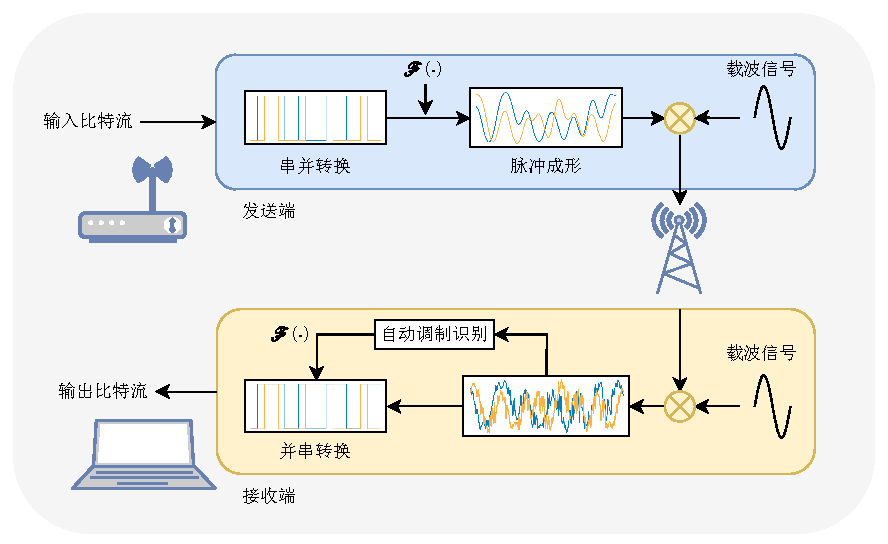
\includegraphics[width=\textwidth]{Image/AMC.pdf}
    \caption{自动调制识别在调制解调过程中的定位}
    \label{fig:AMR}
\end{figure}

随着无线通信技术的快速发展,尤其是在5G和即将到来的6G时代,通信技术正面临着更宽频段的拓展,以获取更多可用的频谱资源\cite{jdid2021machine}。这种需求促进了宽带信号采集技术的进步,特别是对宽频带电磁信号的瞬时采样。这种技术通过捕获宽频带电磁信号的瞬时状态,显著提高了空间电磁信号的捕获概率。然而,要保证信号的完整性,采样频率必须大于信号最高频率的两倍,这根据奈奎斯特采样定理而定。因此,满足宽带电磁频谱感知需求的同时,也带来了更高的硬件代价,如更大的采样速率和更高分辨率的模数转换器,同时也增加了数据处理的复杂性。

在这一背景下,如何在有限的能量和通信资源条件下,有效采集和处理宽带电磁频谱数据,成为了当前通信领域面临的一个重要挑战。自动调制识别作为解决这一挑战的关键技术之一,需同时应对信号的频道检测和调制方式识别,尤其在宽带信号的环境下面临更为复杂的挑战。因此,研究如何提高自动调制识别在宽带通信环境下的性能显得尤为重要。

\subsection{研究意义}\label{sec:background}

在当前的通信技术研究中,自动调制识别技术的重要性日益凸显。传统的自动调制识别算法,尽管在特定情况下有效,却常常受限于低识别准确率和高复杂度。这些局限性源于这些算法对信噪比的高依赖性,以及在处理高维数据时的计算负担。近年来,随着深度学习技术的快速发展和广泛应用,其在自动调制识别领域的应用展示出显著的优势,特别是在提高识别准确性和处理复杂信号方面。

然而,尽管深度学习方法在自动调制识别中取得了显著成果,但仍存在一些挑战和限制。首先,深度学习模型在低信噪比环境下的性能仍然受限。这一问题的根源在于深度学习模型通常需要大量的高质量数据来训练,而在实际应用中,尤其是在复杂或干扰环境中,高质量数据的获取可能非常困难。此外,深度学习模型的复杂性往往较高,这不仅增加了计算资源的需求,也限制了其在资源受限环境中的应用。

目前,自动调制识别领域的研究主要集中在窄带信号的识别上,即仅仅识别信号的调制模式。虽然这在一定程度上提高了通信系统的效率和可靠性,但对于现代通信系统而言,这远远不够。随着5G和预期中的6G技术的发展,宽带通信变得越来越普遍,对宽带信号的处理需求日益增长。在宽带信号的处理中,不仅需要识别信号的调制模式,还需要确定信号占用的子带位置。因此,基于宽带信号的自动调制识别,能够同时识别信号占用的子带位置及其对应的调制模式,成为了一个迫切需要解决的问题。

此外,从更具体的任务角度来看,基于深度学习的宽带调制信号的解调也需要一个更为完善的框架。这不仅涉及到识别子带位置和调制模式,还包括确定符号长度以确认最终调制结果的长度,最终输出宽带调制信号解调后的比特流。这一任务对于提高通信系统的数据传输效率和可靠性至关重要,尤其是在数据量巨大的宽带通信系统中。

结合目前学术界的研究进展,可以看到,虽然深度学习技术已经在自动调制识别领域取得了显著成果,但是在宽带信号处理和解调方面的研究仍处于起步阶段。未来的研究需要关注深度学习模型在低信噪比环境下的性能提升,以及如何减少对大量训练数据的依赖,同时降低模型的复杂度。此外,研究应当更加关注于宽带信号的处理,特别是在确定信号占用的子带位置及其调制模式方面的研究。这不仅将推动自动调制识别技术的发展,也将为未来的宽带通信技术提供重要的技术支撑,从而在更广泛的应用领域中发挥作用。

综上所述,深度学习在自动调制识别领域的应用前景广阔,但仍面临诸多挑战。随着通信技术的不断进步和深度学习技术的持续发展,我们有理由相信这些挑战将被逐步克服,深度学习将在自动调制识别领域发挥更加关键的作用。

% 随着无线通信技术的迅速发展,无线通信设备数量呈指数级增长。据统计预测,未来十年内,无线通信设备数量将增长1000倍。这些设备需时刻传输大量数据,使得频谱资源稀缺的状况更为紧迫。未来的网络中,无线通信系统需要在容量、频谱使用率和能耗效率方面实现10到1000倍的提升。为满足信息时代的万物互联及频谱资源高效利用等应用需求,电磁频谱感知成为信息时代可持续发展的关键。

% 当前,复杂的无线电磁环境对无线通信带来巨大挑战,信号在传输中容易扭曲和畸变,不利于解调。为提高频带利用率和通信速率,出现多种数字调制方式。这增加了接收端解调的难度,尤其在半协同或非协同通信中,接收端需在不知道先验信息的情况下判断调制方式。信号自动调制识别(Automatic Modulation Recognition, AMR)技术研究缓解了这一问题,为信号解调与处理奠定基础,对民用和军用领域都具有高研究价值。

% 信号自动调制识别技术的研究极大缓解了上述问题,自动调制识别介于信号检测与信号解调之间,为后续信号的解调与处理奠定基础。无论在民用还是军用领域都具有很高的研究价值。在民用方面,调制识别可以用于频谱检测和管理,以及识别干扰信号等。在军用领域常用于电子对抗,信息战中需要在截取无线电信息后快速检测其调制方式才能对信息进一步进行解密,也可用于对敌方通信进行干扰以掌握战争对主动权。此外,在主流通信技术中如果能够减少调制方式等先验信息的发送,不仅可以减少额外的频谱资源占用,还可以提高解码效率,降低通信时延。

% 现代5G和6G通信迎来更高更宽的频段拓展,以获取更多可用频谱资源。宽带信号采集技术通过对宽频带电磁信号的瞬时采样抓取,有效提高了空间电磁信号的捕获概率。然而,为保证信号完整性,根据奈奎斯特采样定理,采样频率必须大于信号最高频率的两倍。在满足空间宽带电磁频谱感知需求的同时,采样过程中需投入更高的硬件代价,如更大采样速率和更高分辨率的模数转换器,同时带来更复杂的数据处理。在有限的能量和通信资源下,有效采集宽带电磁频谱数据并在有限资源下实现高效信息压缩与传输,解决大范围下宽带信号的检测识别,是当前亟需解决的基础难题之一。宽带上的自动调制识别面临更为复杂的挑战,需要同时检测信号占用的信道和信号的调制方式。

% 近年来,随着计算机硬件水平的提升,深度学习技术成为焦点。作为机器学习的分支,深度学习以其层次结构和从浅层提取高阶特征的能力在多个领域取得成功。专家开始将深度学习引入通信领域,并发现其在自动调制识别方面表现卓越。

% \dots

% 自动调制识别是复杂电磁环境下信号感知和识别领域中的重要技术。传统的电磁认知识别方法依赖信号采集系统,但由于奈奎斯特采样定理,大数据量采集、传输、存储和处理成为挑战。压缩感知通过使用较小数据量的压缩信号取代奈奎斯特采样信号,极大缓解了信号处理中的瓶颈问题。深度神经网络通过从海量数据中自动提取信号特征,并进行后续识别,为复杂多变的电磁环境中的信号识别问题提供了新的解决方案。因此,基于压缩感知的智能宽带调制识别技术将成为未来研究的关键领域,涵盖宽带信号的压缩采样和调制识别两个方面。

\section{国内外研究现状}
技术领域内,特别是在通讯技术方面,信号调制识别的概念自20世纪初期就开始萌芽。这一时期,通信技术的专家们逐渐认识到,要想解读和理解目标信号中蕴含的关键信息,掌握其调制方式便成了一个不可或缺的步骤。因此,他们开启了针对信号调制方式识别的探索之旅。在最初阶段,这一工作主要依赖于从业人员根据个人经验进行手动识别。这个过程通常包括先对接收到的信号进行降频处理,以将高频信号转化为低频,随后依据信号波形的特定特征或特征组合来推断其调制方式。这种依靠个人判断的方法不仅容易出错,而且极度依赖于从业者的专业经验积累,尤其是在信号的信噪比较低的情况下,通过肉眼观察进行识别显得尤为困难。

随着移动通信技术的发展和现代战争模式的变化,信号调制识别的重要性日益凸显,促使更多的专业人士投入到这一领域的研究中,从而加速了相关技术的进步。特别是在20世纪60年代末期,斯坦福大学的Weaver及其团队的一项关键技术报告标志着自动调制识别技术的重大突破。这份报告首次向公众展示了如何应用模式识别技术来迅速且自动地鉴别高频无线电信号的调制类型,开启了自动调制分类技术的新纪元\cite{weaver1969automatic}。通过对信号频谱的数字化分析及利用最近邻模式识别器进行分类,实现了高精度的调制方式识别,这一研究成果奠定了自动调制识别研究的基础。

自那以后,自动调制识别技术的研究主要围绕两大核心方向展开:一方面是基于决策理论的最大似然假设检验方法;另一方面是采用基于特征提取的统计模式识别算法。此外,随着深度学习技术的快速发展,基于深度学习的调制识别算法也正受到广泛关注并处于积极研究阶段。这些技术的进步不仅极大提升了信号解调的速度和准确性,也为通信技术领域的发展开辟了新的道路。
\subsection{传统方法}
\subsubsection{似然比法}

决策理论基础上的似然假设检验法,根植于概率论这一学科土壤,将调制方式的识别过程转化为一系列多重假设的检验问题。在此框架下,当接收端捕获到信号后,便开始对该信号中未知的目标参数进行建模,以便获得这些参数的概率分布特性。接着,基于特定的似然标准,构建似然函数,并为每种可能的调制方式假设计算对应的似然值。最终,依托贝叶斯信息标准(Bayesian Information Criterion, BIC)并在一定的阈值限制之下,选择似然值最高的调制方式作为对目标信号调制方式的预测。图\ref{fig:likelihood}以直观的方式呈现了基于似然比假设检验的调制识别过程的主要步骤。

\begin{figure}
    \centering
    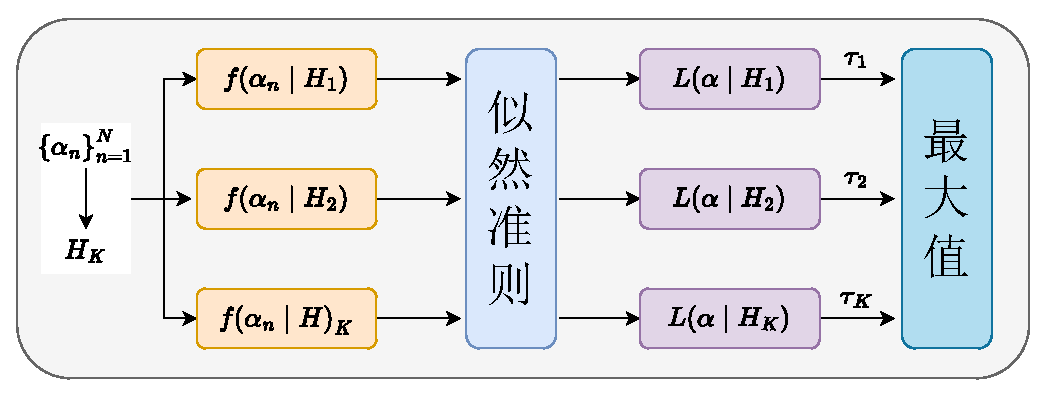
\includegraphics[width=\textwidth]{Image/likelihood.pdf}
    \caption{基于似然比检验的调制识别过程}
    \label{fig:likelihood}
\end{figure}

在基于似然比检验的调制识别方法的早期尝试中,尽管研究者们努力寻找最佳的分类规则,但长时间内成效有限。然而,在1988年,Kim和Polydoros的工作带来了一次飞跃,他们提出了一种名为平均似然比检验(Average Likelihood Ratio Test, ALRT)的算法\cite{kim1988digital}。此算法在高斯信道条件下,以调制信号的相位信息为基础,通过平均化处理构建似然函数,对BPSK和QPSK信号展现出优异的分类性能。1995年,Huang和Polydoros在ALRT算法的基础上进行了优化\cite{huan1995likelihood},提出了一种新型的准对数似然比(Quasi Log Likelihood Ratio, QLLR)分类器,不仅提高了MPSK信号的识别准确率,还扩展了算法的应用范围,覆盖了所有二维信号类型。通过对MQAM信号的研究,Yang等人\cite{yang1998log}证明了在信噪比高于12dB的条件下,ALRT算法能够实现100\%的识别率。进一步地,文献\cite{sills1999maximum}通过利用最大似然算法,成功实现了MPSK和MQAM信号的联合分类,并探究了在相干与非相干条件下分类性能的差异。

1998年,Boiteau等人引入了一种新的算法框架,即广义似然比检验(Generalized Likelihood Ratio Test, GLRT)\cite{boiteau1998general}。与ALRT算法相比,GLRT算法处理信号参数作为确定性未知变量,无需对信号或信道参数进行任何假设,减少了算法对信号先验知识的依赖,从而适用于更广泛的环境,并简化了算法复杂度。2000年,Panagiotou和Anastasopoulos在ALRT和GLRT的基础上,提出了混合似然比检验(Hierarchical Likelihood Ratio Test, HLRT)算法\cite{panagiotou2000likelihood},该算法能够根据多个未知参数进行建模,并根据不同参数采用不同的判决标准来构建似然函数,显示出对非恒包络调制信号有更高的识别性能。

近年来,决策理论下的调制识别算法研究持续深入。2013年,靳晓燕等研究人员提出一种新颖的通过查表方式简化最大似然算法的计算过程\cite{靳晓艳2013一种最大似然调制识别的快速算法},显著降低计算复杂度,使之适用于接收机进行实时信号处理。2015年,一项基于压缩感知框架的最大似然调制识别算法被提出\cite{童年2015非重构压缩样值的},能够在较少的数据量下实现更精确的识别结果。2016年,吴斌等人\cite{吴斌2016基于记忆因子的连续相位调制信号最大似然调制识别}利用最大似然算法构建记忆因子,应用于连续相位调制信号的识别中。最新的研究进展中,一种适用于多输入多输出(Multiple Input Multiple Output, MIMO)通信系统的最大似然识别算法被开发,该算法基于ALRT准则,构建了独立于天线数目和信道状况的似然函数,展现了增加天线数目有助于提升识别精度。在未知载波频率和符号速率的情况下,文献\cite{zhu2018likelihood}成功实现了MPSK和MQAM信号的有效分类。此外,一种在平坦衰落信道中有效工作的最大似然估计器也在文献\cite{chen2019faster}中提出。

\subsubsection{特征提取法}

基于特征提取的统计模式识别算法由于其强大的实用价值和相对简单的工程部署能力而受到广泛关注。这种方法的应用主要遵循三个核心步骤:信号预处理、特征提取、以及最终的分类器识别,其中特征提取阶段是整个过程中的关键。在信号预处理阶段,通过对信号执行一系列简单变换,例如滤波和降频处理,使信号规范化,降低了后续数据处理的复杂性。这个过程还包括清洗和筛选信号数据,以确保去除那些可能干扰识别准确性的非理想数据元素。图\ref{fig:feature_based}展示了基于特征提取的调制识别过程的主要步骤。

\begin{figure}
    \centering
    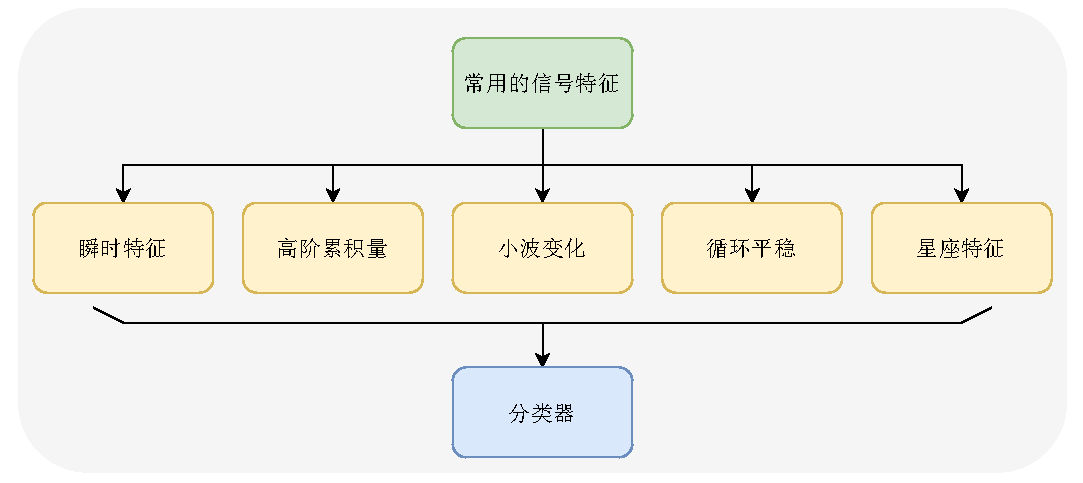
\includegraphics[width=\textwidth]{Image/feature.pdf}
    \caption{基于特征提取的调制识别过程}
    \label{fig:feature_based}
\end{figure}

特征提取阶段致力于在多个维度中发掘出不同调制方式之间的显著差异,由于不同特征可能反映出同一调制方式的不同调制信息,因此特征选择对于优化识别结果具有决定性影响。进而,在分类器识别阶段,通过利用精心挑选的特征,分类器能够有效区分不同的调制信号,这对于通信系统的效率和可靠性至关重要。

\subsubsection{瞬时特征法}
瞬时特征作为信号分析领域中的一种常用特征表示方法,因其获取便利性而广泛应用于信号调制识别。这些特征主要涵盖信号的幅度、相位和频率等方面。Nandi等人\cite{nandi1995automatic}开发出了多种基于瞬时特征的新方法,以实现对各种模拟信号的有效分类,并且在特定信噪比下达到了高达90\%的识别成功率。此外,在文献\cite{陈怀新2004基于统计特征主分量的信号调制识别}中主成分分析法等技术被用来对瞬时特征进行压缩,减少特征的维度,从而提升了调制识别的效率和精度。
\subsubsection{高阶累积量法}

高阶累积量作为一种反映信号统计特性的重要方法,特别是在抵抗高斯有色噪声方面显示出其独特的优势。信号的高阶统计特征被作为一种创新的特征参数用于信号调制识别,这一方法在低信噪比条件下也能实现可靠的识别性能。

\subsubsection{小波变换法}
小波变换技术因其在处理非平稳信号方面的有效性而在调制识别中占据了一席之地。通过小波变换得到的信号特征,尤其是那些能够揭示信号时频信息的特征,被文献\cite{刘明骞2018认知无线电}证明能够成功识别出不同的信号调制类型。此外,文献\cite{li2019wavelet}使用小波变换结合主成分分析和神经网络等先进技术在数字信号识别的准确度方面取得了显著提升。

\subsubsection{循环平稳特征法}
循环平稳特征利用信号的循环谱特性来区分不同的调制方式,有效地抑制了高斯噪声并揭示了调制相关的相位和频率信息。这些特征在处理多径信道条件下的信号识别问题时显示出了良好的性能。

\subsubsection{星座图特征}
星座图特征通过分析信号的星座图来直观地展现不同调制类型之间的差异,为调制识别提供了一个有效的途径。通过从星座图中提取的特定特征,结合先进的算法和技术,能够在不同信噪比条件下准确区分不同的调制信号。

\subsubsection{分类器选择}
最后,在选择合适的分类器方面,不同的机器学习算法可以根据其特点和应用场景的需求来优化调制识别过程。支持向量机、决策树、随机森林、最近邻分类器以及神经网络等,都是在不同数据规模和分类任务中常见的选择。神经网络特别适用于大规模数据训练,通过复杂的网络结构和大量的参数调整,可以建立复杂数据和分类结果之间的深层次联系,从而在分类任务中取得优异的表现。

\subsection{深度学习方法}
深度学习技术的快速发展为通信领域带来了创新的研究方向和解决方案,尤其在信号调制识别任务中表现出巨大的潜力和优势。不同于传统调制识别方法那样依赖于手工特征提取,深度学习算法通过其深层网络结构自动探索和学习数据中的复杂特征,无需人工干预即可挖掘出信号的本质特性。得益于大数据时代的到来,深度学习算法能够处理大量数据,通过这些数据训练出性能优异的识别模型。随着多个调制识别相关开源数据集的公开\cite{o2016convolutional}\cite{o2018over}及自动调制识别技术在军事及民用通信领域的广泛部署,近年来,深度学习驱动的自动调制识别技术受到了广泛关注。本节将对近年来深度学习在自动调制识别领域的研究进展进行综述。

卷积神经网络(Convolution Neural Network, CNN)模型展现了在处理具备空间属性数据(如图像分割、目标检测及分类)方面的显著优势。自动调制识别研究亦纳入CNN,借助其卓越的空间特征提取能力识别信号调制类型。根据输入数据的不同,基于CNN的自动调制识别模型分为两大类:一类是直接以原始I/Q数据为输入的CNN模型,另一类则处理经过预先处理的输入。除此此外,还有针对高效CNN架构的研究,旨在满足现代通信系统对延迟和复杂性的严格要求。

使用原始I/Q信号作为输入数据的CNN模型:2016年,采用简易四层CNN模型处理I/Q数据的方法初次被探讨,显示出超越多数传统方法的识别准确性\cite{o2016convolutional}。随后,Tekbıyık等人通过调整层数或超参数,提出了改进版CNN模型\cite{tekbiyik2020robust}。鉴于简单CNN架构可能未能充分提取I/Q信号中的代表性特征,进一步采用了复杂层次结构或变换操作的改进CNN模型,Liu等人受ImageNet 2015赛事获奖架构启发,提出基于残差网络(ResNet)和密集连接网络(DenseNet)的新型DL-AMR模型,以有效传递多层次学习特征至分类模块\cite{liu2017deep}。Zhang等人开发了一种实时信号调制分类模型,采用三级跳转残差网络识别调制信号,尽管识别准确性有所提高,但计算复杂性亦显著增加\cite{zhang2021real}。由于许多神经网络基模型直接借鉴于计算机视觉任务,这忽视了通信信号的固有属性。为解决此限制,Yashashwi等人提出在输入CNN模型前,估算接收信号的载波频率偏移和相位噪声,通过训练可调函数计算相位和频率偏移(校正参数),以减少偏移影响\cite{yashashwi2018learnable}。

使用预处理后的I/Q信号作为输入数据的CNN模型:由于原始信号经射频链路多环节处理及信道影响会丧失一些重要特性,如高阶累积量、频谱图和星座图等,直接使用原始I/Q信号作为输入的CNN模型的性能有限。而结合传统特征提取方法与CNN模型将有效地解决这一痛点,如Zeng等人通过短时离散傅立叶变换将一维无线电信号转化为频谱图像,进而通过高斯滤波降低噪声,提出的谱卷积网络模型实现了优于基准模型的识别准确率\cite{zeng2019spectrum}。Li等人提出的双谱-AlexNet方法将双谱的幅值谱输入CNN,有效抑制白噪声影响\cite{li2019automatic}。为提高非高斯噪声下识别性能,Ma等人引入循环相关熵谱,采用ResNet进行分类\cite{ma2019automatic}。此外,星座图作为AMR中另一广泛使用信号表示方法,可以从中直接提取特征确定调制方案。Peng等人将星座图转为3通道图像\cite{peng2018modulation},利用CNN模型处理彩色图像的能力进行分类。需要注意的是,正交幅度调制(QAM)模式间的混淆问题十分严重,为解决此问题,Wang等人采用两个CNN模型提升识别准确率,并分别以I/Q数据和星座图为训练数据\cite{wang2019data}。其中,基于星座图的CNN主要用于区分16QAM与64QAM的混淆问题。为充分利用循环谱图像的抗噪性和星座图提供的高阶调制识别能力,Wu等人设计了双分支CNN,提取多种特征后进行融合分类\cite{wu2019convolutional}。采用特征融合理念,Zhang等人实施了一种多模态融合模型,该模型结合了神经网络提取的不同图像特征与8个手工提取特征,以获得更区分度高的特征\cite{zhang2019automatic}。其他如眼图\cite{wang2017modulation}、特征点图像\cite{lee2019feature}及方形特征矩阵\cite{chen2021signet}等不同的输入信号表示形式也被尝试应用于自动调制识别模型中。

高效CNN架构设计:为满足超五代通信系统的预期延迟要求,Hermawan等人通过在每层中使用较少滤波器且减少可训练参数总数,开发了改进的基于CNN的自动调制识别模型\cite{hermawan2020cnn}。该模型处理时间低于0.01ms,符合超五代通信要求,尽管可训练参数数量减少,但仍保持较高的识别准确率。为应对5G业务对超高可靠性和低延迟的需求,Huynh-The等人提出了一种高效CNN模型,该模型在每个卷积块中并行采用多种非对称卷积核,并在网络中采用残差连接\cite{huynh2020mcnet}。Shi等人通过采用挤压-激励(Squeeze-and-Excitation, SE)块引入通道注意机制,实现了另一种更轻量级的模型\cite{shi2022combining}。

循环神经网络(Recurrent Neural Network, RNN)模型:无线通信信号除携带空间相关特性外,通常还包含时间相关特征,RNN模型则能很好捕捉序列中的时间关系。近年来,基于RNN的模型结构在自动调制识别领域取得良好性能,如Hong等人提出的基于RNN的AMR方法,利用GRU实现了优于部分CNN模型的识别准确率\cite{hong2017automatic}。Rajendran等人将I/Q信号转换为幅值和相位后输入到长短期记忆(LSTM)网络,实现高识别准确率\cite{rajendran2018deep}。以上仅使用两层RNN的模型已展现出在自动调制识别任务中的优异性能,证明了RNN在提取通信信号时间特征方面的能力。Ke等人设计了一个LSTM去噪自编码器,采用紧凑的RNN架构获取信号调制方案,在低成本计算平台上易于实现,同时达到了先进水平\cite{ke2021real}。

除了CNN和RNN模型外,近年来,随着Transfomer在自然语言处理领域的成功应用,也有研究者尝试将其应用于自动调制识别任务中。\cite{hamidi2021mcformer}提出了一种新颖的,基于Transformer的自动调制识别,利用其自注意力机制来捕捉信号中的长距离依赖关系,并于卷积神经网络所提取的特征进行对比和研究。文献\cite{tonchev2022automatic}中,作者利用图卷积神经网络(Graph Convolutional Network, GCN)探讨了各种调制模式之间的时间频域特征。

\section{本文主要贡献与创新}\label{sec:background}

\subsection{本文研究内容}\label{sec:background}

本论文延伸并深化了自动调制识别领域的研究,特别是在基于深度学习的宽带信号调制识别和调制解调技术方面。研究的意义可以从以下三个方面进行阐述:

1. 基于深度学习的自动调制识别:本论文致力于进一步提高调制识别的准确率和降低计算复杂度。通过应用深度学习模型,本文旨在更有效处理复杂的信号特征,提升在复杂无线电环境中的调制识别性能。这对于高效的通信技术发展提供了重要的技术支持。

2. 基于深度学习的宽带信号调制识别:本论文专注于宽带信号中占用的子带位置及其对应的调制模式的识别。这一研究不仅拓宽了自动调制识别的应用范围,也对于解决宽带信号处理中的新挑战,如频谱感知和频谱分配优化,具有至关重要的意义。通过深度学习技术的应用,能够有效识别并处理宽带信号中的多种调制模式,从而提升通信系统的灵活性和效率。

3. 基于深度学习的宽带信号调制解调:本论文还研究了宽带信号的调制解调过程,包括识别子带位置、调制模式和符号长度,进而输出宽带调制信号解调后的比特流。这一部分的研究不仅提升了调制识别的准确性和效率,而且实现了从信号检测到信息恢复的完整流程,极大提升了宽带信号处理的实用性和灵活性。

总体来说,本论文在基于深度学习的自动调制识别技术的基础上,通过拓展到宽带信号的识别和解调,开辟了通信技术在更广阔领域内应用的新视角,为未来通信系统的发展提供了新的可能性和解决方案。

\subsection{本文研究创新点}\label{sec:background}

本研究致力于解决宽带信号处理中的几个关键问题,主要集中在信号调制识别、宽带信号的信道识别与调制识别、以及宽带信号的解调三个方面。研究内容包括自适应噪声矫正模块的开发,多陪集采样的应用,以及利用神经网络进行宽带信号解调的创新性工作。

1. 提升自动调制识别在低信噪比下的准确率

在信号调制识别方面,本研究引入了一种先进的自适应噪声矫正模块,旨在缓解噪声对信号识别准确性的负面影响。该模块采用动态调整机制,根据环境噪声水平的实时变化,自动调节矫正强度,从而提高信号调制识别的鲁棒性。这一模块的引入,显著提升了在多变和复杂噪声环境下的信号调制识别系统性能,提高了不同调制模式的区分能力。

2. 实现宽带信号调制识别与信道识别

针对宽带信号处理中的采样挑战,本研究采用了多陪集采样策略,目的是提升宽带信号的采样效率,并全面捕捉其频谱信息。此外,本研究采用了基于神经网络的方法,实现了对宽带信号的信道识别与调制识别的高效处理。所提出的神经网络模型能够同时处理信号的信道占用和调制模式识别任务,为宽带信号的高效分析提供了一种新的途径。

3. 为宽带信号解调提供一个完整的框架

在宽带信号的解调阶段,本研究提出了一套综合性解决方案。在完成信道与调制识别的基础上,研究重点转向如何有效提取信号对应的比特流。经过深入的研究和创新设计,我们开发了一种有效的宽带信号解调算法,使系统能够准确而高效地重构原始信号的信息,满足现实世界应用中对数据准确性和传输效率的严格要求。

总体而言,本文通过研发自适应噪声矫正模块、应用多陪集采样技术对宽带信号进行采样和利用神经网络进行信号识别解调,全面探索了宽带信号处理的关键问题,并在信号调制识别、信道与调制识别、以及宽带信号解调等多个方面取得了较好成果。未来,我们计划深化这些研究,进一步优化这些技术,以适应日益发展的通信技术和不断变化的通信环境。同时,我们鼓励对这些技术在实际应用场景中进行更广泛的验证和探索,以确保它们在真实环境中的有效性和可靠性。

\section{论文结构}\label{sec:background}
本论文共分为五章,各章节内容安排如下:

本论文深入研究了自动调制识别与解调技术,在六个章节中系统地阐述了相关理论、实践方法及其创新点。以下为每个章节的简介:

第一章:绪论

本章介绍了研究的背景和意义,着重指出了自动调制识别技术在现代通信系统中的重要性。论文概述了自动调制识别与解调技术的研究现状,包括传统方法和近年来兴起的深度学习方法。此外,本章还阐明了本文的主要研究内容和结构安排,为读者提供了研究的总体框架和研究方向。

第二章:调制识别的理论基础

本章详细介绍了调制识别的理论基础,包括基本的调制原理、信号模型及其特性。本章还讨论了传统的调制识别技术,如特征提取法和似然比法,以及这些技术的局限性。此章节为理解后续章节中提出的方法奠定了坚实的理论基础。

第三章:窄带信号调制识别

本章中,提出了一种创新的自适应噪声矫正的针对窄带信号的调制识别网络。该章节详细介绍了网络的设计思想、结构以及工作原理。此外,还阐述了如何通过自适应调整来优化噪声矫正效果,从而在复杂噪声环境下提高调制识别的准确性和鲁棒性。

第四章:宽带信号调制识别与信道识别及解调

本章专注于宽带信号的处理,特别是调制识别与信道识别的问题。本章探讨了宽带信号特有的挑战,如高采样率和数据处理的复杂性,并介绍了采用多陪集采样等技术应对这些挑战的方法。深入研究了宽带信号的识别与解调过程。本章详细描述了如何从宽带信号中提取有效信息并进行准确的解调,以得到原始信号的比特流。此外,本章还讨论了神经网络在宽带信号解调中的应用及其优势。

第五章:总结与展望

在最后一章中,本文总结了整个研究的主要成果和贡献。同时,对研究中存在的局限性和未来可能的研究方向进行了讨论。本章为整个研究提供了一个全面的回顾,并对未来自动调制识别技术的发展趋势提出了展望。

\begin{figure}[htbp]
    \centering
    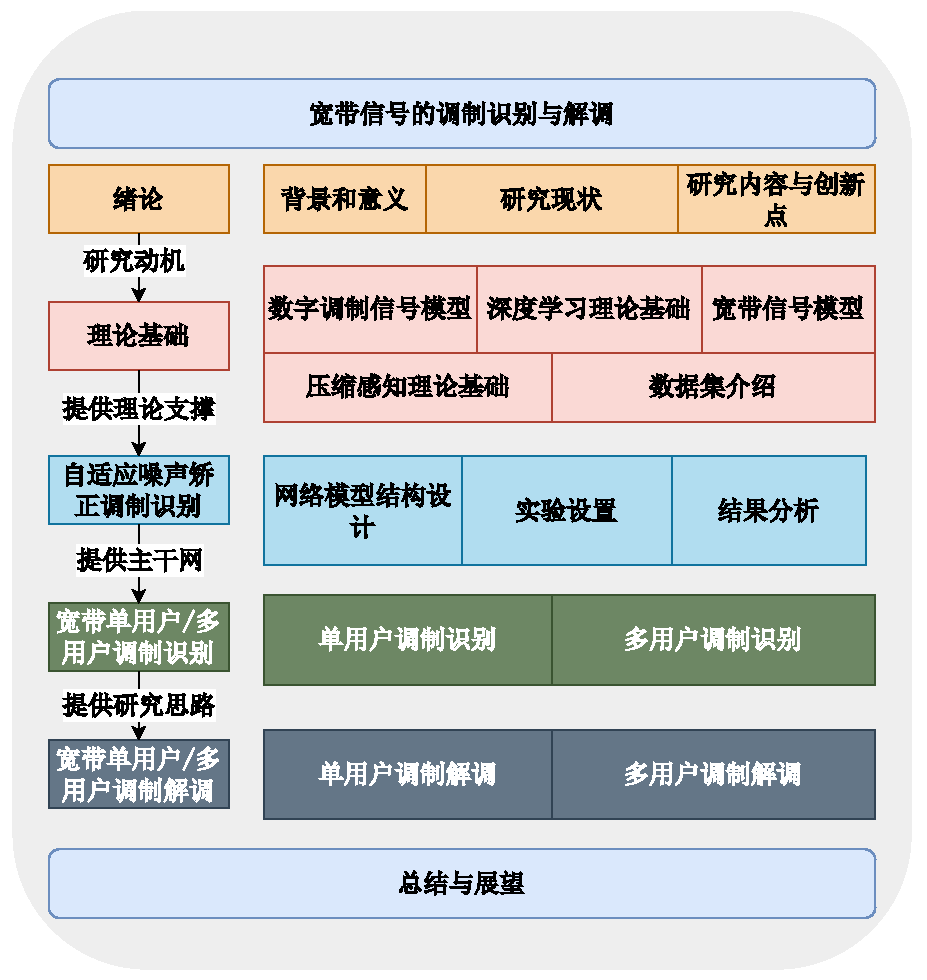
\includegraphics[width=\textwidth]{Image/chap1_overallstructure.pdf}
    \caption{论文结构}
    \label{fig:thesis_structure}
\end{figure}
